\documentclass[stu,12pt,a4paper,floatsintext]{apa7}
\usepackage{graphicx}
\usepackage{float}
\usepackage{booktabs}
\usepackage{xcolor}
\usepackage{listings}
\usepackage{amsmath}
\usepackage{hyperref}

% Monospace listing style for depth maps
\lstset{
  basicstyle=\ttfamily\scriptsize,
  frame=single,
  backgroundcolor=\color[gray]{0.97},
  breaklines=false,
  columns=fixed,
  keepspaces=true,
}

\title{LLMs Mind's Eye: Text Based Depth Representations as Spatial Reasoning Scaffolds}
\author{Robert Paszek}
\affiliation{Department of Cognitive Science and Artificial Intelligence, Tilburg University}
\course{Research Workshop}
\professor{Supervisor: Bruno Nicenboim}
\duedate{April 12, 2025}

\begin{document}
\maketitle

% ═══ MOTIVATION ═══
\section*{Research Motivation}

Large language models (LLMs) excel at mathematical proofs, code generation, and logical deduction, yet they consistently fail at spatial reasoning. On the ARC\nobreakdash-AGI\nobreakdash-2 benchmark, pure LLMs score 0\% and the best reasoning system (OpenAI's o3) reaches only 4\%, while humans average 60\% \cite{chollet2025}. Perspective taking accuracy for GPT\nobreakdash-4o from the human viewpoint is just 27.5\% \cite{shiri2024}. Bigger models, multimodal training, and chain of thought prompting have not closed this gap.

This failure matters beyond benchmarks. Autonomous vehicle perception errors have caused fatal accidents when systems misclassified pedestrians \cite{ntsb2019}. Of 49 FDA cleared surgical robots, none operates above Level~3 autonomy \cite{lee2024}, partly because autonomous soft tissue manipulation remains in its infancy \cite{khanna2025}. LLMs can reason through logic, but they collapse when reasoning requires understanding 3D structure.

The standard approach is adding vision modules. SpatialVLM generates spatial reasoning training data through depth estimation \cite{chen2024spatialvlm}. SpatialVLA injects 3D position encodings into vision language action models \cite{qu2025spatialvla}. These approaches work, but they increase model complexity and keep models dependent on visual input. There is an under explored alternative: LLMs might already have the reasoning capability they need. What they lack is the right \emph{representation format} for spatial information.

This idea builds on Larkin and Simon \cite{larkin1987}, who demonstrated that diagrams make certain problems easier to solve, not by adding new information, but by making spatial relationships computationally accessible. The same principle could apply to LLMs: structured, spatially organized text instead of raw natural language may be sufficient to unlock spatial reasoning.

% ═══ RESEARCH QUESTION ═══
\section*{Research Question}

\begin{center}
\emph{To what extent do text based depth representations, generated from a voxel domain specific language, improve large language model performance on spatial reasoning tasks where current models score below 50\%?}
\end{center}

% ═══ BACKGROUND ═══
\section*{Background}

The theoretical foundation comes from Larkin and Simon \cite{larkin1987}. They demonstrated that the computational difference between sentential and diagrammatic representations is not about information content. It is structural. Diagrams group spatially related information together, which enables perceptual operations that are computationally expensive in plain text. This principle suggests that converting spatial problems into structured, spatially organized text could give LLMs similar benefits.

Recent work has started exploring spatial intermediates for LLM reasoning. The Visualization of Thought (VoT) framework showed that generating spatial intermediates (ASCII like grids) during reasoning improved LLM performance on navigation and tiling tasks \cite{wu2024}. The Whiteboard of Thought (WoT) paradigm demonstrated that a draw, render, perceive loop (where models generate visual code, render it, and interpret the output) improved spatial accuracy over pure text reasoning \cite{menon2024}. VoxPoser used LLMs to generate Python code that filled 3D voxel grids with affordance values for robot planning, achieving zero shot generalization \cite{huang2023}.

But no existing system implements a complete closed loop. One where an LLM writes 3D spatial code, receives text based depth feedback from a raycasting camera system, verifies its reasoning against the rendered output, and iteratively revises. All without any vision model. The Mind's Eye system, which this proposal aims to evaluate, implements precisely this architecture. It uses VOXI, a voxel description language, paired with a text based raycaster that produces ASCII depth maps (digits 0 to 9 representing distance from camera). Figure~\ref{fig:feedback} shows the feedback mechanism.

% ═══ FIGURE 1: Compact 5-view pairs ═══
\begin{figure}[H]
\centering

% FRONT
\begin{minipage}[c]{0.28\textwidth}
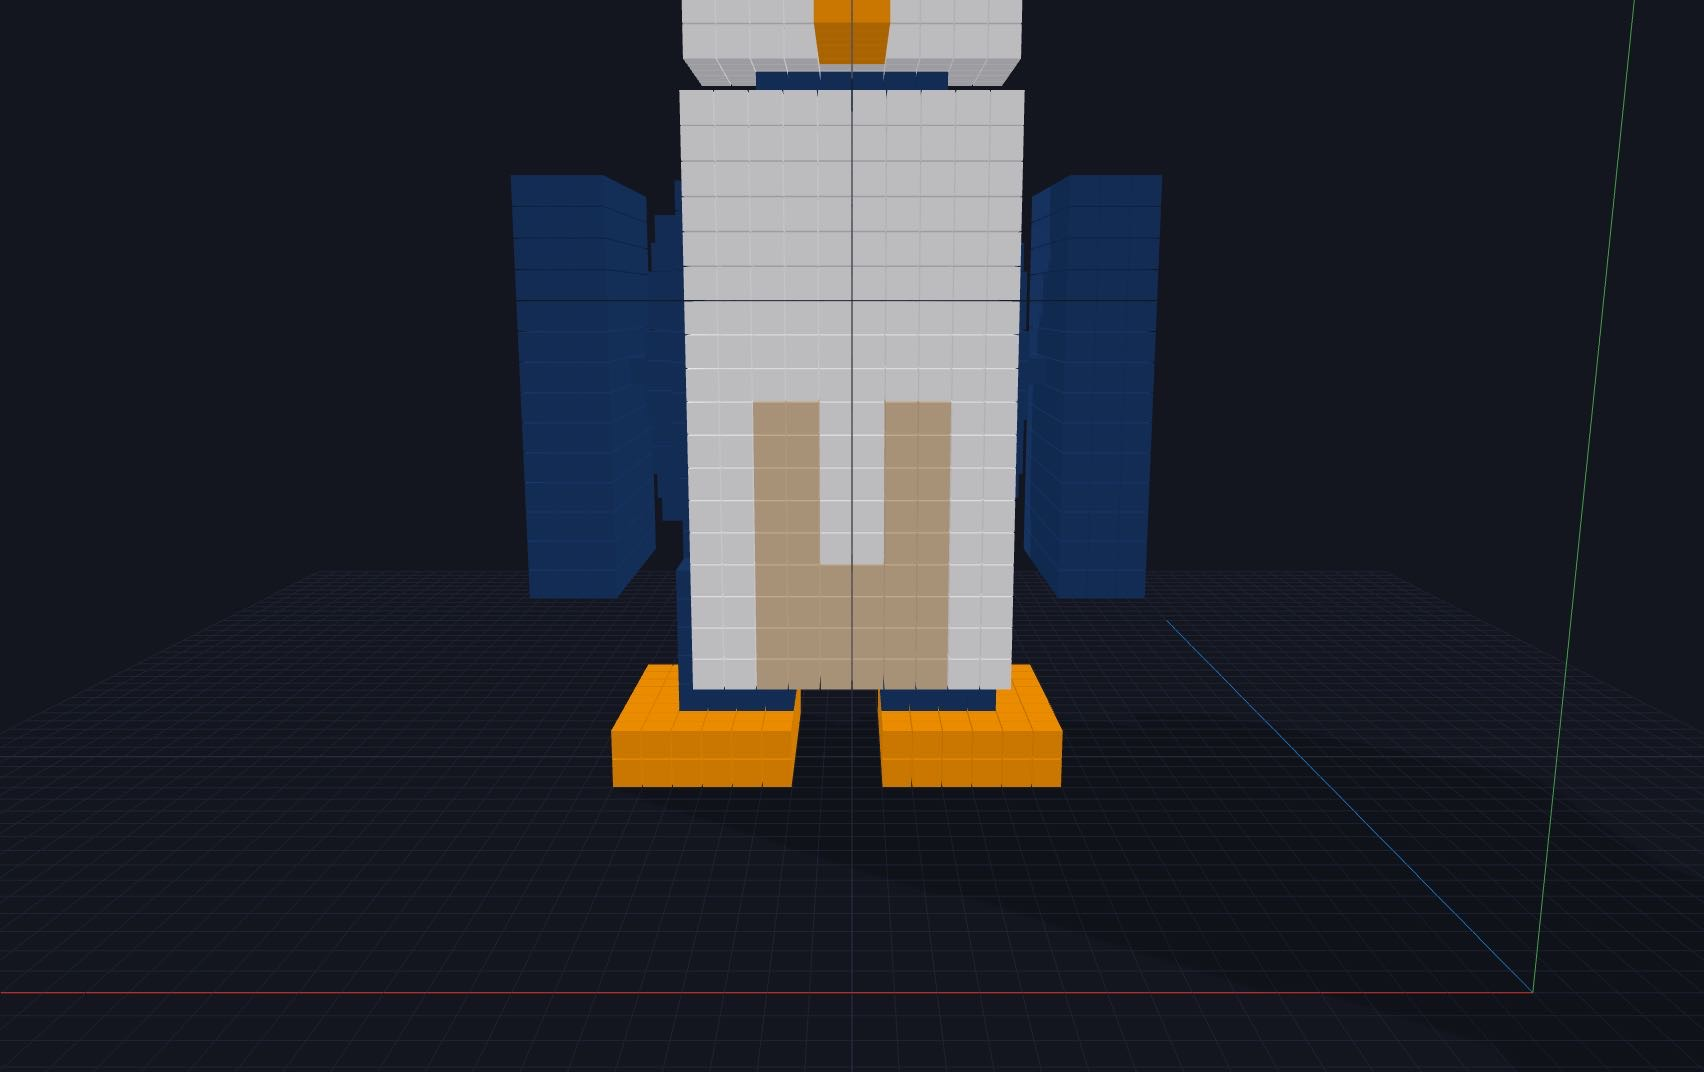
\includegraphics[width=\textwidth]{proposal-assets/penguin-render-front.jpg}
\end{minipage}%
\hfill
\begin{minipage}[c]{0.68\textwidth}
\begin{lstlisting}
FRONT (->X, ^Y) 32x32   .=empty 0=near 9=far
 0 . . . . . . . . . . . . 5 5 4 4 4 4 4 5 5 . . . . . . . . . . .
 3 . . . . . . . . . . . 3 3 3 2 2 2 2 3 3 3 5 . . . . . . . . . .
 9 . . . . . . . . . . . . . 4 4 4 4 4 4 6 . . . . . . . . . . . .
12 . . . . . . 4 4 4 . . 3 3 3 3 3 3 3 3 3 3 5 . . 4 4 4 . . . . .
18 . . . . . . 4 4 4 6 5 3 3 3 3 3 3 3 3 3 3 4 5 6 4 4 4 . . . . .
27 . . . . . . . . . . . 3 3 3 3 3 3 3 3 3 3 4 . . . . . . . . . .
31 . . . . . . . . . 4 4 4 4 4 4 . . . 4 4 4 4 4 4 . . . . . . . .
\end{lstlisting}
\end{minipage}

\vspace{6pt}

% RIGHT
\begin{minipage}[c]{0.28\textwidth}
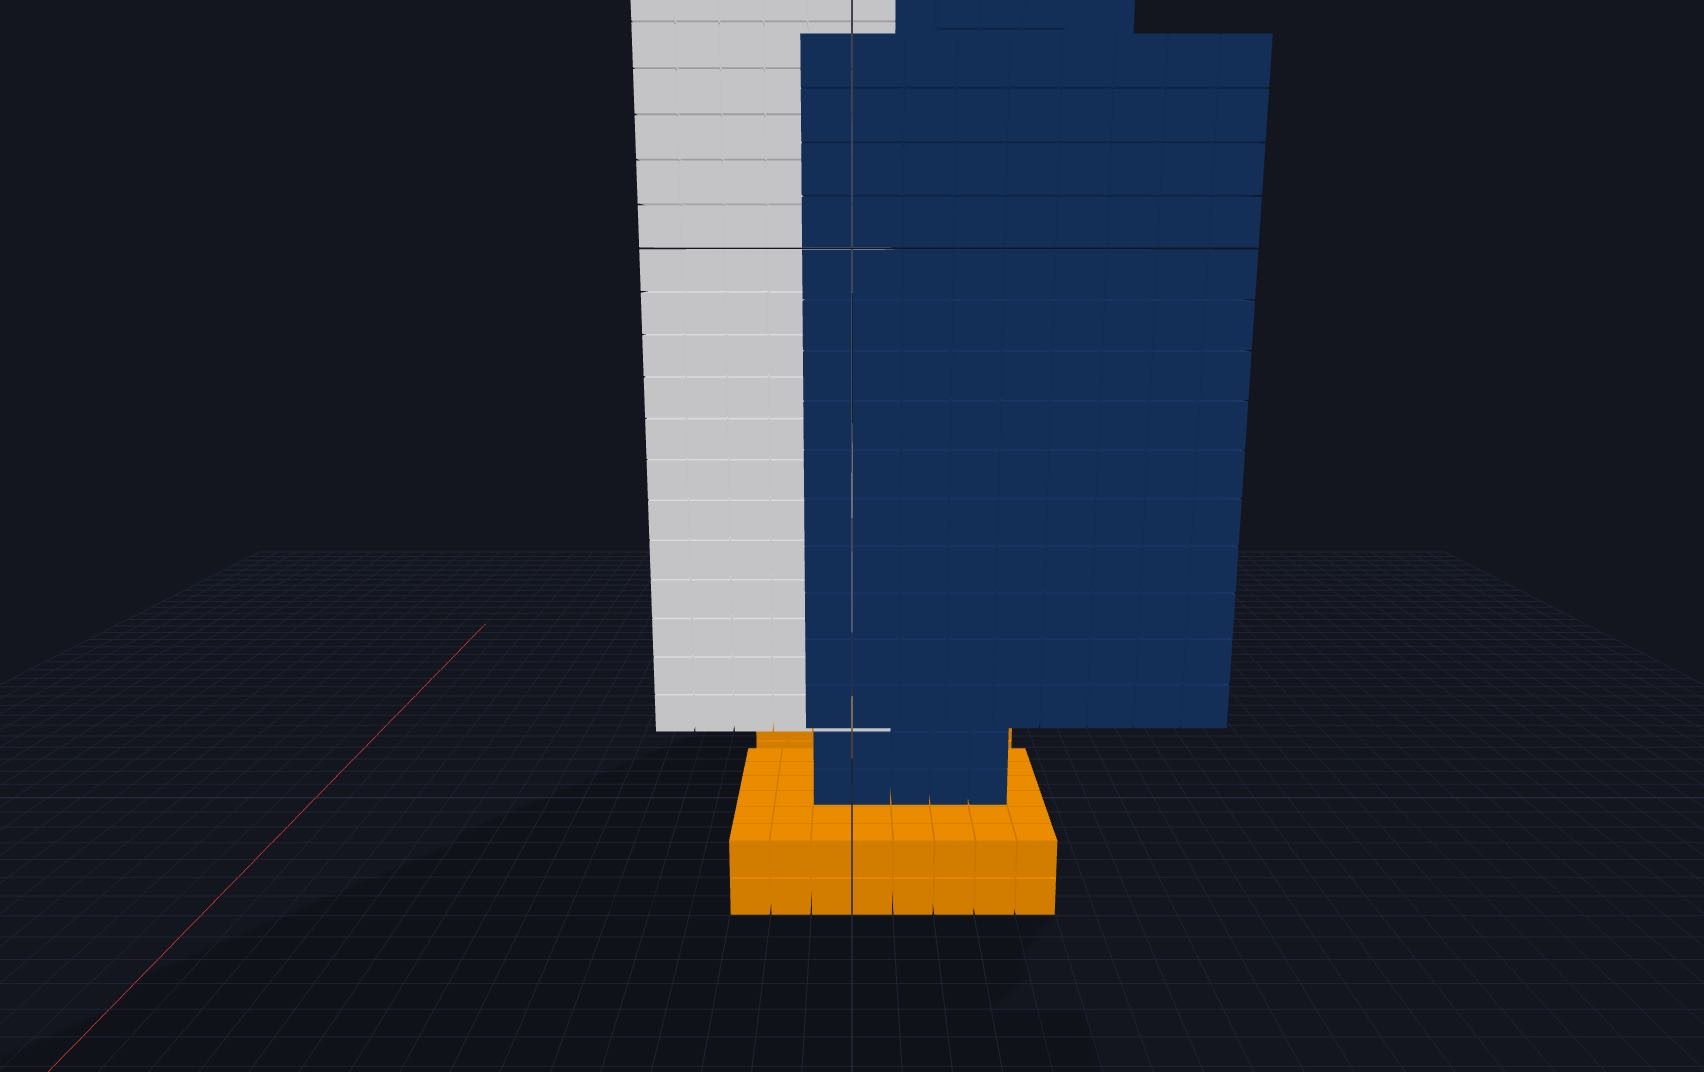
\includegraphics[width=\textwidth]{proposal-assets/penguin-render-right.jpg}
\end{minipage}%
\hfill
\begin{minipage}[c]{0.68\textwidth}
\begin{lstlisting}
RIGHT (->Z, ^Y) 32x32   .=empty 0=near 9=far
 0 . . . . . . . . . . . . . . 4 4 3 3 3 3 3 4 4 . . . . . . . . .
 9 . . . . . . . . . . . . . . 4 4 4 4 4 3 4 4 . . . . . . . . . .
12 . . . . . . . . . . . 3 3 3 3 1 1 1 1 1 1 1 1 1 . . . . . . . .
18 . . . . . . . . . . . 3 3 3 3 1 1 1 1 1 1 1 1 1 3 4 . . . . . .
27 . . . . . . . . . . . 3 3 3 3 3 3 3 3 3 4 4 . . . . . . . . . .
31 . . . . . . . . . . . . . 2 2 2 2 2 2 2 2 . . . . . . . . . . .
\end{lstlisting}
\end{minipage}

\vspace{6pt}

% BACK
\begin{minipage}[c]{0.28\textwidth}
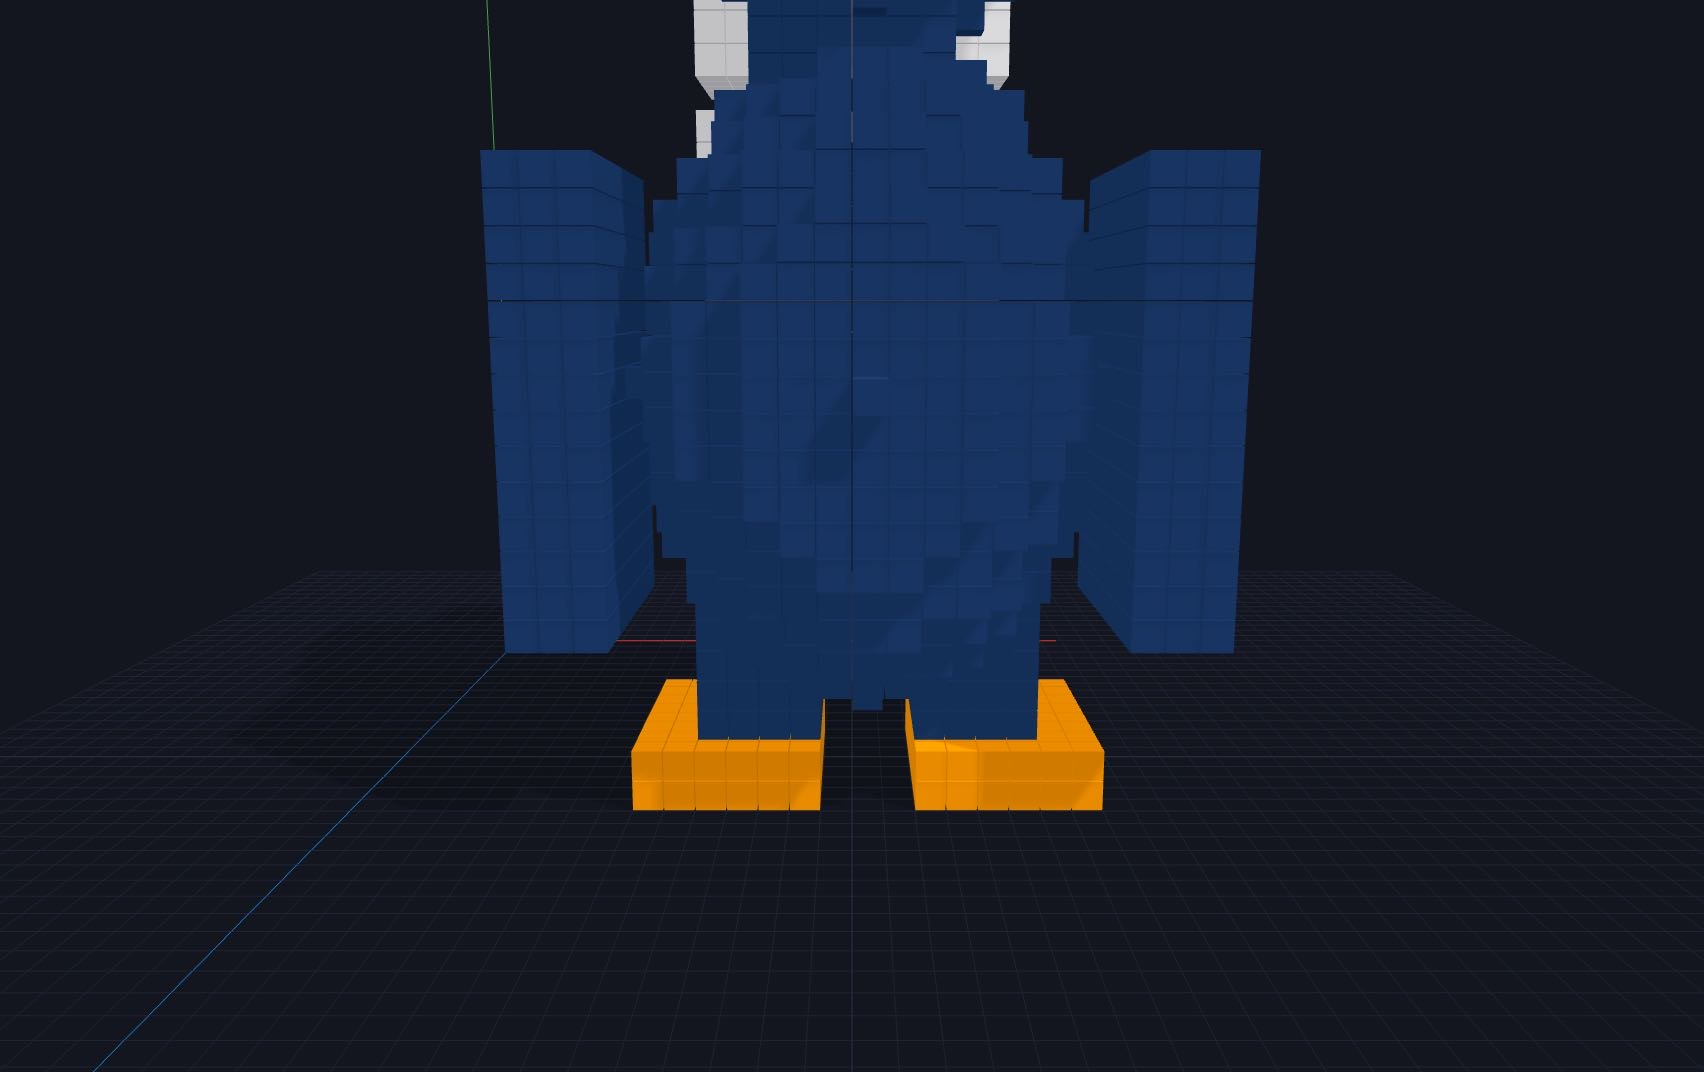
\includegraphics[width=\textwidth]{proposal-assets/penguin-render-back.jpg}
\end{minipage}%
\hfill
\begin{minipage}[c]{0.68\textwidth}
\begin{lstlisting}
BACK (->X, ^Y) 32x32    .=empty 0=near 9=far
 0 . . . . . . . . . . . 4 3 3 3 3 3 3 3 4 . . . . . . . . . . . .
 9 . . . . . . . . . . . . 3 3 3 3 3 3 3 . . . . . . . . . . . . .
12 . . . . . 2 2 2 . . 3 3 2 2 2 2 2 2 2 3 3 . . 2 2 2 . . . . . .
18 . . . . . 2 2 2 3 3 2 2 2 2 2 2 2 2 2 2 2 3 3 2 2 2 . . . . . .
27 . . . . . . . . . . 3 3 3 3 3 3 3 3 3 3 3 . . . . . . . . . . .
31 . . . . . . . . 3 3 3 3 3 3 . . . 3 3 3 3 3 3 . . . . . . . . .
\end{lstlisting}
\end{minipage}

\vspace{6pt}

% LEFT
\begin{minipage}[c]{0.28\textwidth}
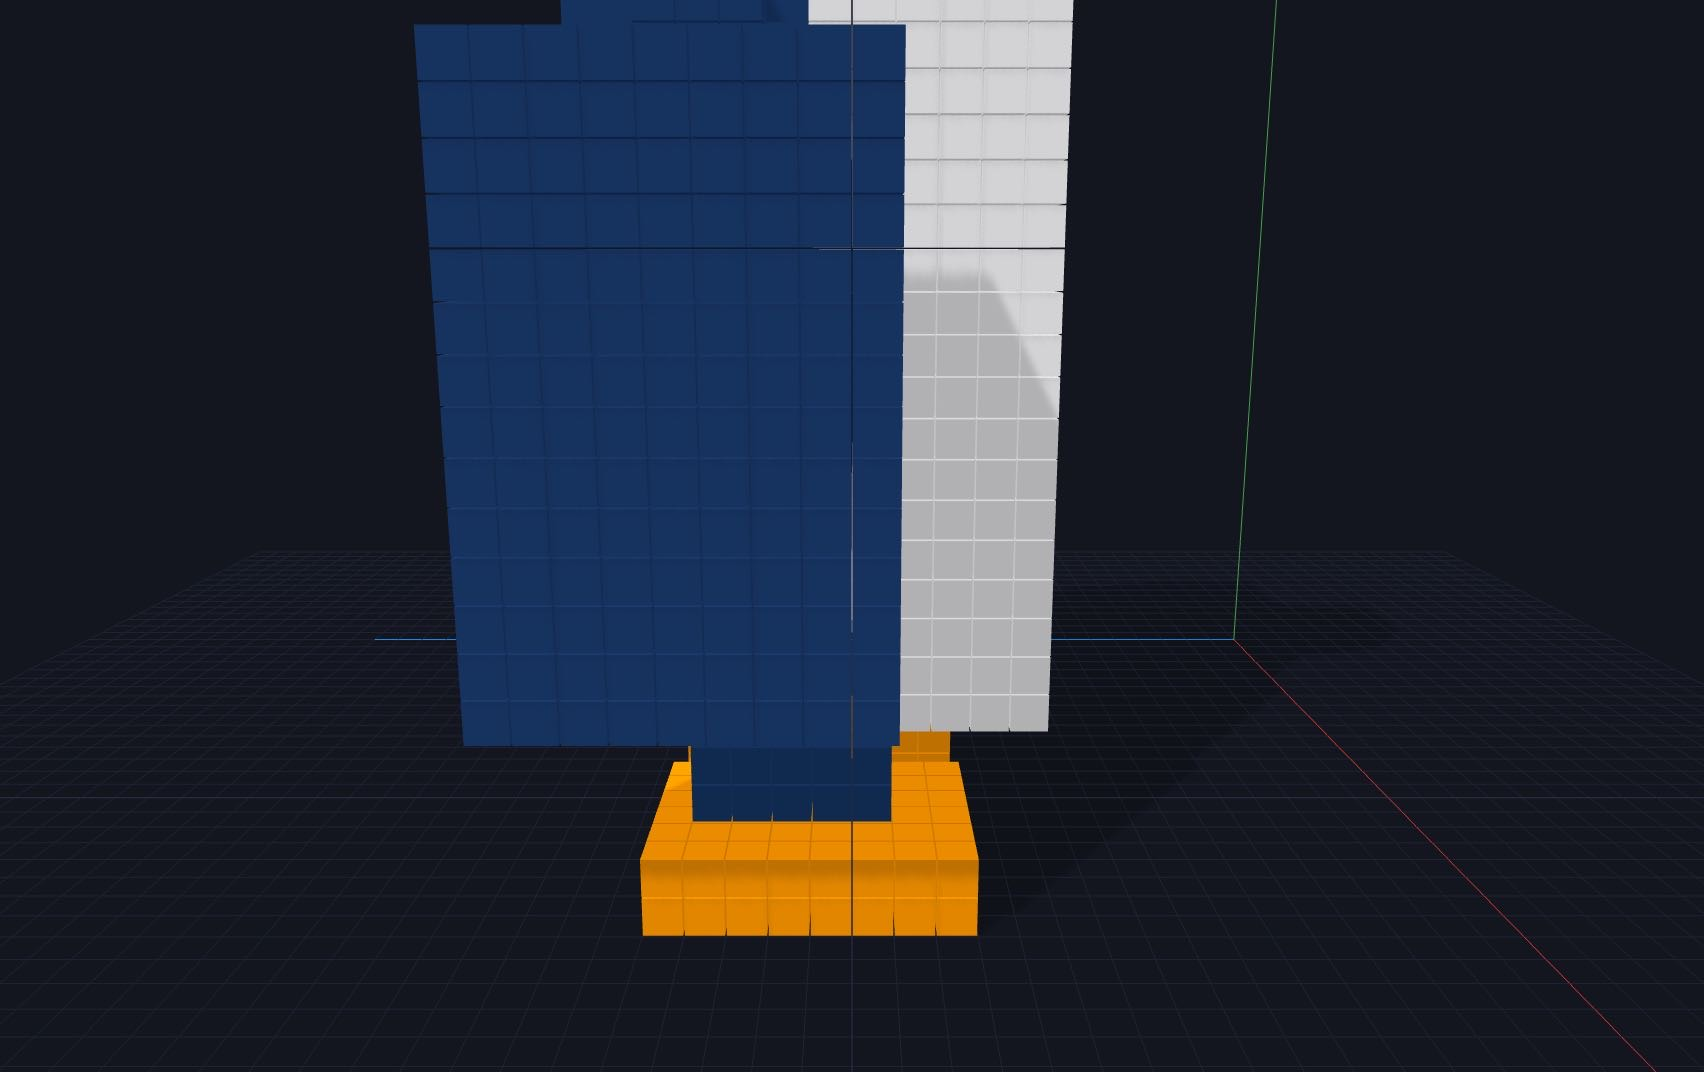
\includegraphics[width=\textwidth]{proposal-assets/penguin-render-left.jpg}
\end{minipage}%
\hfill
\begin{minipage}[c]{0.68\textwidth}
\begin{lstlisting}
LEFT (->Z, ^Y) 32x32    .=empty 0=near 9=far
 0 . . . . . . . . . 5 4 4 4 3 4 4 4 5 . . . . . . . . . . . . . .
 9 . . . . . . . . . . 4 4 4 4 4 4 4 4 . . . . . . . . . . . . . .
12 . . . . . . . . 2 2 2 2 2 2 2 2 2 3 3 3 3 . . . . . . . . . . .
18 . . . . . . 5 4 2 2 2 2 2 2 2 2 2 3 3 3 3 . . . . . . . . . . .
27 . . . . . . . . . . 4 4 3 3 3 3 3 3 3 3 3 . . . . . . . . . . .
31 . . . . . . . . . . . 3 3 3 3 3 3 3 3 . . . . . . . . . . . . .
\end{lstlisting}
\end{minipage}

\vspace{6pt}

% TOP
\begin{minipage}[c]{0.28\textwidth}
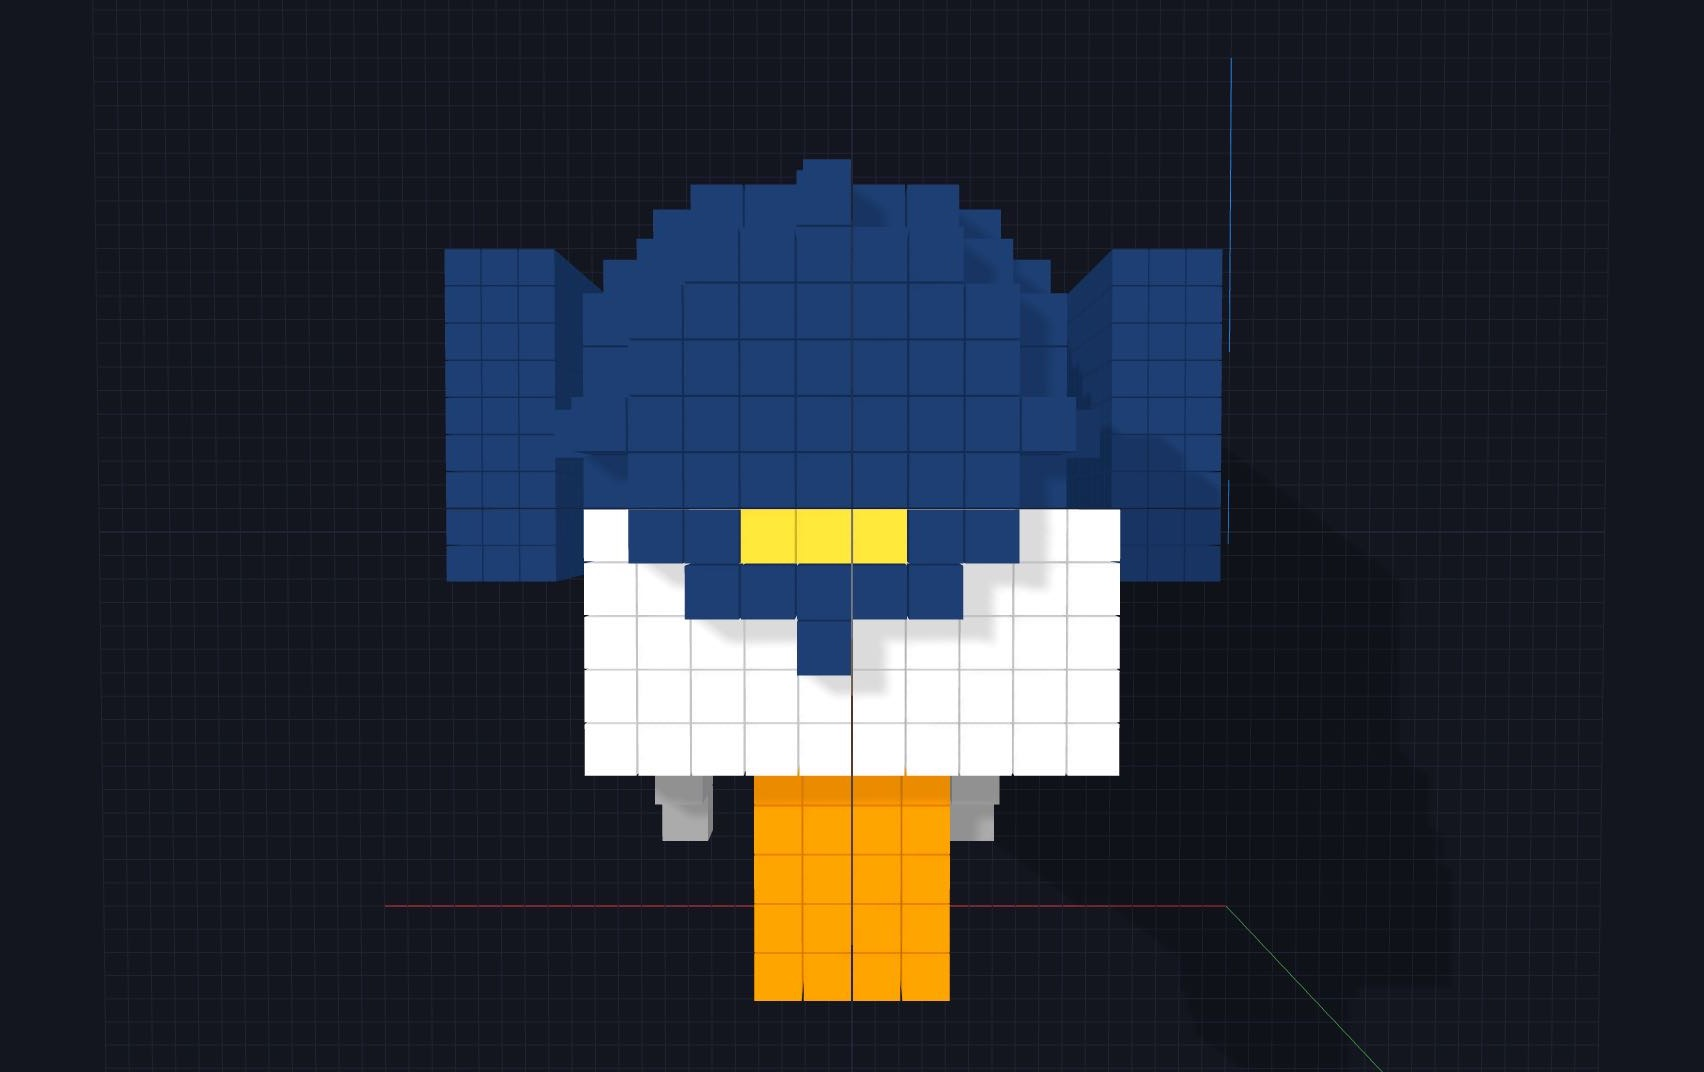
\includegraphics[width=\textwidth]{proposal-assets/penguin-render-top.jpg}
\end{minipage}%
\hfill
\begin{minipage}[c]{0.68\textwidth}
\begin{lstlisting}
TOP (->X, ^Z) 32x32     .=empty 0=near 9=far
 8 . . . . . . 3 3 3 . . 5 4 3 3 3 1 3 3 3 4 5 . . 3 3 3 . . . . .
 9 . . . . . . 3 3 3 . 5 4 3 1 0 0 0 0 0 1 3 4 5 . 3 3 3 . . . . .
11 . . . . . . 3 3 3 9 4 3 0 0 0 0 0 0 0 0 0 3 4 9 3 3 3 . . . . .
17 . . . . . . . . . 9 9 0 0 0 0 0 0 0 0 0 0 9 9 9 . . . . . . . .
19 . . . . . . . . . . . 0 0 0 0 0 0 0 0 0 0 . . . . . . . . . . .
21 . . . . . . . . . . . . . 1 1 1 1 1 . 1 . . . . . . . . . . . .
\end{lstlisting}
\end{minipage}

\caption{The Mind's Eye feedback mechanism applied to a voxel penguin (32$\times$32$\times$32). Left column: 3D WebGL renders from five orthographic cameras. Right column: the corresponding text based depth maps the LLM reads. Each digit (0 to 9) encodes ray traced distance from the virtual camera. The LLM receives only the text. No vision model is involved. Full resolution maps in the Appendix.}
\label{fig:feedback}
\end{figure}

% ═══ METHODS ═══
\section*{Methods}

\subsection*{Experimental Design}

The experiment follows a 2$\times$2 factorial design. The first factor is \emph{representation type}: natural language only versus natural language augmented with text based depth matrices. The second factor is \emph{model capability}: a stronger model (Claude Sonnet) versus a weaker one (Claude Haiku). The dependent variable is accuracy, the percentage of spatial reasoning questions answered correctly.

\subsection*{Datasets}

Three benchmarks will be used:

\begin{enumerate}
\item \textbf{SpartQA} \cite{mirzaee2021}: multi hop spatial reasoning questions from text scene descriptions (e.g., inferring the relation between block A and block C through block B). Twenty tasks of varying difficulty will be sampled.

\item \textbf{CATER} \cite{girdhar2020}: synthetic video scenes rendered with the CLEVR engine, requiring spatial tracking of object movement and occlusion in 3D. Five tasks covering object counting, motion tracking, and occlusion detection will be used.

\item \textbf{VOXI scenes}: thirty procedurally generated 3D scenes (16$\times$16$\times$16 grids, seed=42) with five question types: collision detection, relative position, motion direction, object count, and closer to camera judgments.
\end{enumerate}

\subsection*{Feature Extraction}

In the depth matrix condition, the Mind's Eye system renders each scene into six text based depth maps (front, back, left, right, top, bottom) via orthographic raycasting. Each cell in the grid contains a digit 0 to 9 representing normalized distance from the camera. For CATER video, Depth Anything V2 produces per frame 20$\times$20 depth matrices quantized to the same range. In the control condition, models receive only the original text descriptions or VOXI source code without depth rendering.

\subsection*{Procedure}

Each model and condition combination is tested on all tasks. The LLM receives the problem description and, in the depth condition, the corresponding depth matrices. It produces a single pass answer with no iterative refinement, which is then compared against the ground truth.

\subsection*{Statistical Analysis}

A two way ANOVA will test the main effects of representation type and model capability, and their interaction. Preliminary results suggest depth matrices help stronger models but may hurt weaker ones, making the interaction effect theoretically interesting.

Post hoc comparisons (Tukey's HSD) will identify significant pairwise differences. Accuracy will also be broken down by task type to identify which spatial subtasks benefit most. Effect sizes (Cohen's \emph{d}) will be reported for all significant comparisons.

% ═══ REFERENCES ═══
\newpage
\begin{thebibliography}{9}

\bibitem[Chen et al., 2024]{chen2024spatialvlm}
Chen, B., Xu, Z., Kirmani, S., Ichter, B., Sadigh, D., Guibas, L., \& Xia, F. (2024). SpatialVLM: Endowing vision-language models with spatial reasoning capabilities. \emph{Proceedings of the IEEE/CVF Conference on Computer Vision and Pattern Recognition (CVPR)}.

\bibitem[Chollet et al., 2025]{chollet2025}
Chollet, F., Knoop, M., Kamradt, G., Landers, B., \& Pinkard, H. (2025). ARC-AGI-2: A new challenge for frontier AI reasoning systems. \emph{ARC Prize Foundation}. Retrieved from \url{https://arcprize.org/blog/announcing-arc-agi-2-and-arc-prize-2025}

\bibitem[Girdhar \& Ramanan, 2020]{girdhar2020}
Girdhar, R., \& Ramanan, D. (2020). CATER: A diagnostic dataset for compositional actions and temporal reasoning. \emph{International Conference on Learning Representations}.

\bibitem[Huang et al., 2023]{huang2023}
Huang, W., Wang, C., Zhang, R., Li, Y., Wu, J., \& Fei-Fei, L. (2023). VoxPoser: Composable 3D value maps for robotic manipulation with language models. \emph{Conference on Robot Learning}.

\bibitem[Larkin \& Simon, 1987]{larkin1987}
Larkin, J. H., \& Simon, H. A. (1987). Why a diagram is (sometimes) worth ten thousand words. \emph{Cognitive Science, 11}(1), 65--100. \url{https://doi.org/10.1111/j.1551-6708.1987.tb00863.x}

\bibitem[Mirzaee et al., 2021]{mirzaee2021}
Mirzaee, R., Faghihi, H. R., Ning, Q., \& Kordjamshidi, P. (2021). SpartQA: A textual question answering benchmark for spatial reasoning. \emph{Proceedings of the 2021 Conference of the North American Chapter of the Association for Computational Linguistics: Human Language Technologies} (pp. 4582--4598). \url{https://aclanthology.org/2021.naacl-main.364/}

\bibitem[Khanna et al., 2025]{khanna2025}
Khanna, R., Raison, N., Granados Martinez, A., Ourselin, S., Montorsi, F., Briganti, A., \& Dasgupta, P. (2025). At the cutting edge: The potential of autonomous surgery and challenges faced. \emph{BMJ Surgery, Interventions, \& Health Technologies, 7}(1), e000338. \url{https://doi.org/10.1136/bmjsit-2024-000338}

\bibitem[Lee et al., 2024]{lee2024}
Lee, A., Baker, T. S., Bederson, J. B., \& Rapoport, B. I. (2024). Levels of autonomy in FDA-cleared surgical robots: A systematic review. \emph{npj Digital Medicine, 7}, 103. \url{https://doi.org/10.1038/s41746-024-01102-y}

\bibitem[Menon et al., 2024]{menon2024}
Menon, S., Zemel, R., \& Vondrick, C. (2024). Whiteboard-of-thought: Thinking step-by-step across modalities. \emph{arXiv preprint arXiv:2406.14562}.

\bibitem[{National Transportation Safety Board}, 2019]{ntsb2019}
{National Transportation Safety Board}. (2019). \emph{Collision between vehicle controlled by developmental automated driving system and pedestrian, Tempe, Arizona, March 18, 2018} (Highway Accident Report NTSB/HAR-19/03). Washington, DC.

\bibitem[Shiri et al., 2024]{shiri2024}
Shiri, F., Guo, X.-Y., Far, M. G., Yu, X., Haffari, G., \& Li, Y.-F. (2024). An empirical analysis on spatial reasoning capabilities of large multimodal models. \emph{Proceedings of the 2024 Conference on Empirical Methods in Natural Language Processing (EMNLP)}.

\bibitem[Wu et al., 2024]{wu2024}
Wu, W., Mao, S., Zhang, Y., Xia, Y., Dong, L., Cui, L., \& Wei, F. (2024). Visualization-of-thought elicits spatial reasoning in large language models. \emph{Advances in Neural Information Processing Systems 38 (NeurIPS 2024)}.

\bibitem[Qu et al., 2025]{qu2025spatialvla}
Qu, D., Song, H., Chen, Q., Yao, Y., Ye, X., Ding, Y., Wang, Z., Gu, J., Zhao, B., Wang, D., \& Li, X. (2025). SpatialVLA: Exploring spatial representations for visual-language-action model. \emph{arXiv preprint arXiv:2501.15830}.

\end{thebibliography}

% ═══ APPENDIX ═══
\newpage
\begin{center}
{\large\bfseries Appendix: Full Resolution Mind's Eye Depth Maps}\\[6pt]
\normalsize Voxel Penguin Model (32$\times$32$\times$32), 5 Orthographic Views\\
Left: 3D WebGL render. Right: text based depth map (what the LLM reads).\\
\textbf{No vision model is used. The LLM receives only the text.}\\[6pt]
\small\textbf{Depth encoding:} \texttt{.} = empty \quad \texttt{0} = closest to camera \quad \texttt{1} to \texttt{8} = progressively deeper \quad \texttt{9} = farthest
\end{center}

\vspace{12pt}

% FRONT
\noindent\textbf{FRONT View}\\[-4pt]
\rule{\textwidth}{0.4pt}

\noindent
\begin{minipage}[t]{0.45\textwidth}
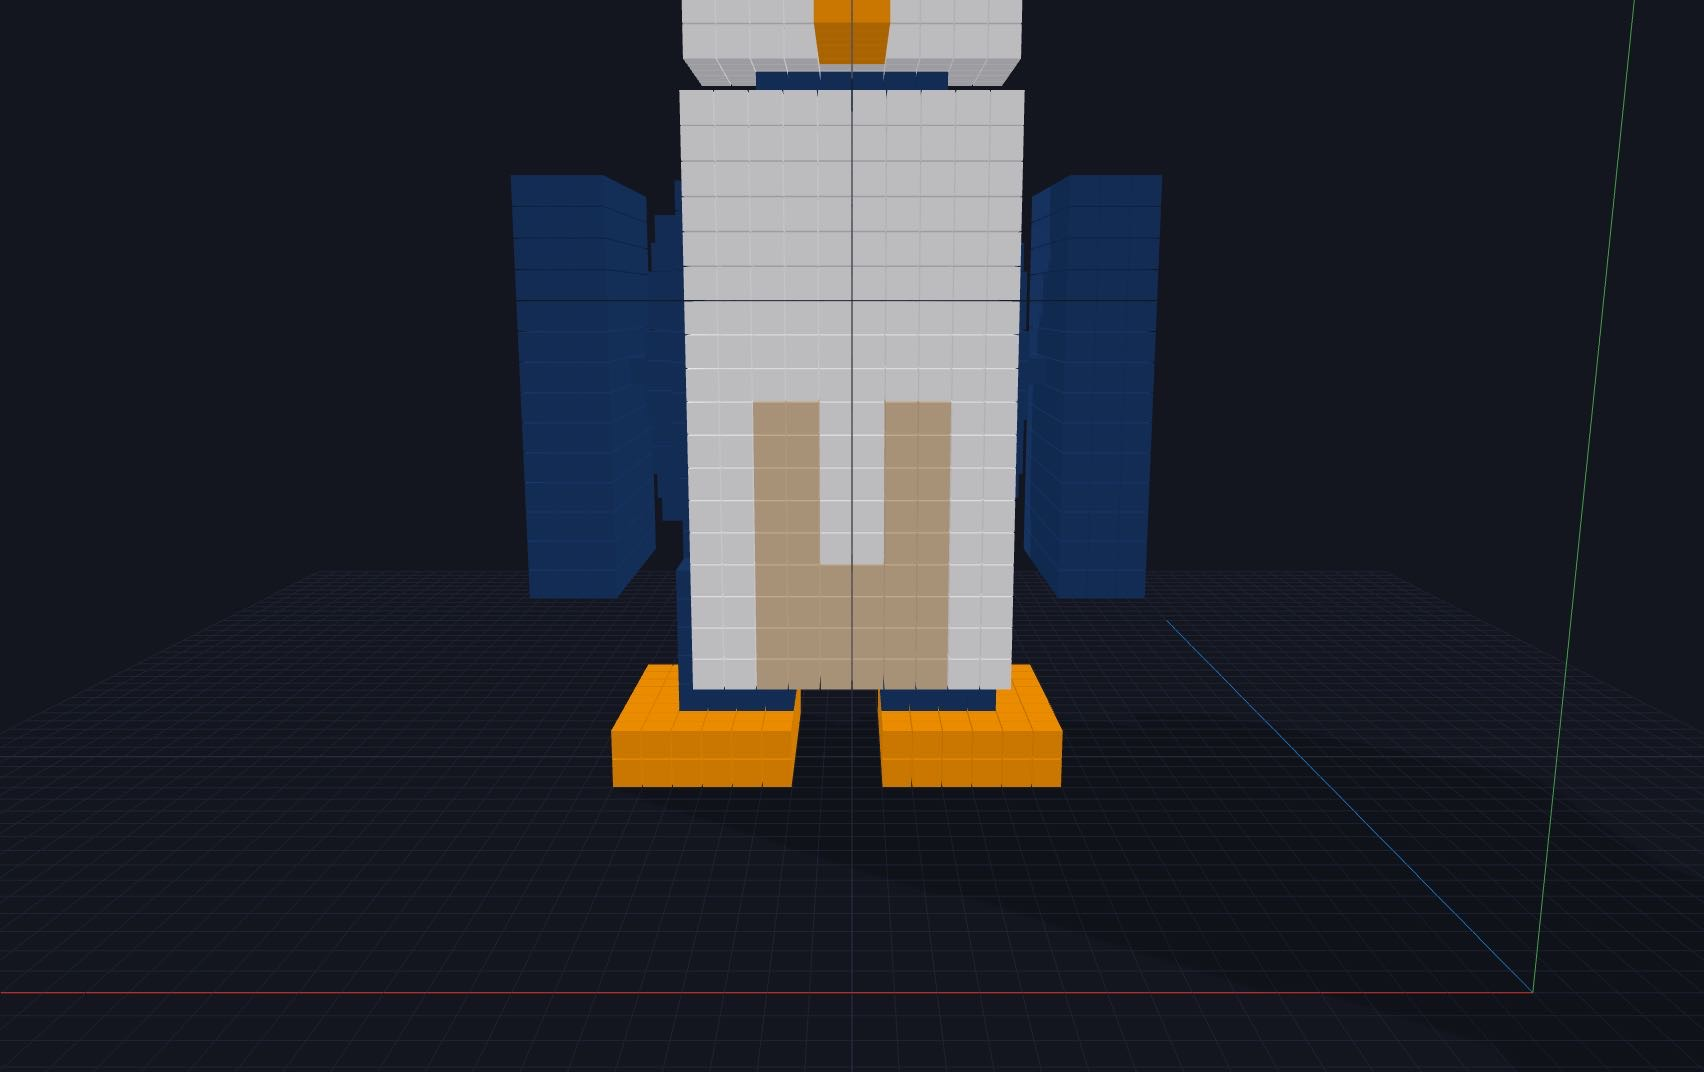
\includegraphics[width=\textwidth]{proposal-assets/penguin-render-front.jpg}
\end{minipage}%
\hfill
\begin{minipage}[t]{0.52\textwidth}
\lstinputlisting[basicstyle=\ttfamily\fontsize{5}{6}\selectfont]{proposal-assets/penguin-full-front.txt}
\end{minipage}

\vspace{8pt}

% RIGHT
\noindent\textbf{RIGHT View}\\[-4pt]
\rule{\textwidth}{0.4pt}

\noindent
\begin{minipage}[t]{0.45\textwidth}
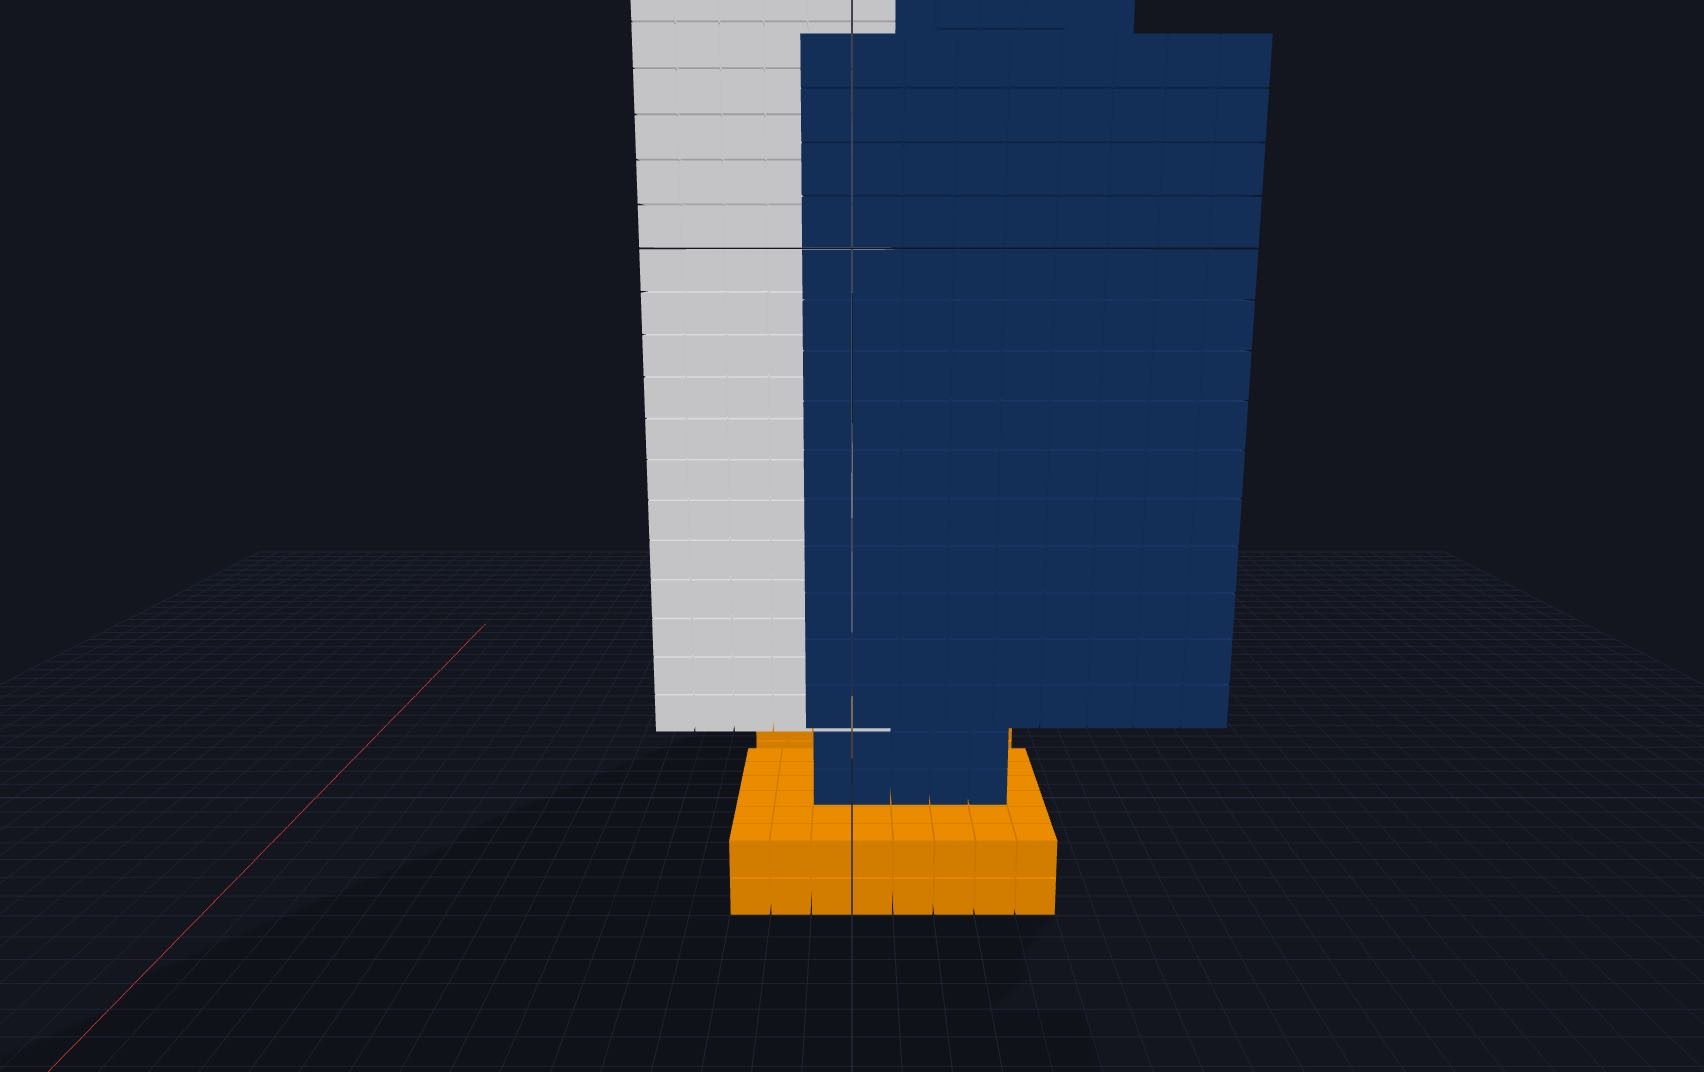
\includegraphics[width=\textwidth]{proposal-assets/penguin-render-right.jpg}
\end{minipage}%
\hfill
\begin{minipage}[t]{0.52\textwidth}
\lstinputlisting[basicstyle=\ttfamily\fontsize{5}{6}\selectfont]{proposal-assets/penguin-full-right.txt}
\end{minipage}

\vspace{8pt}

% BACK
\noindent\textbf{BACK View}\\[-4pt]
\rule{\textwidth}{0.4pt}

\noindent
\begin{minipage}[t]{0.45\textwidth}
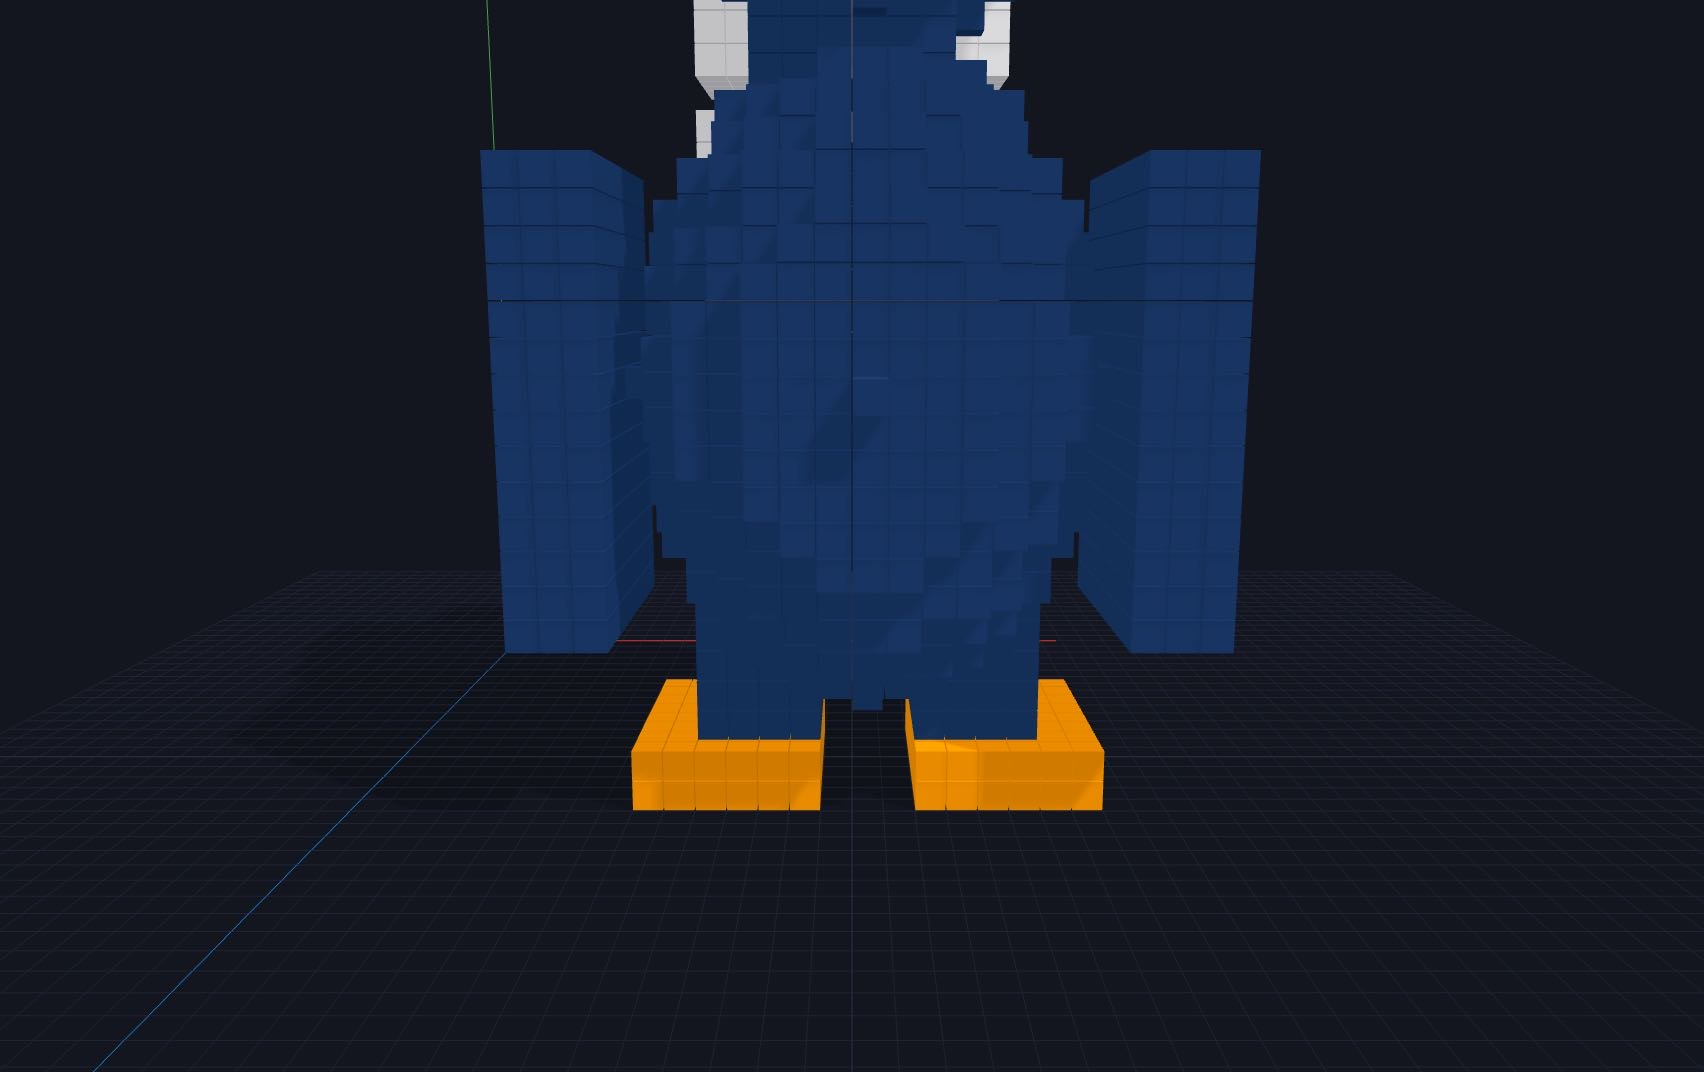
\includegraphics[width=\textwidth]{proposal-assets/penguin-render-back.jpg}
\end{minipage}%
\hfill
\begin{minipage}[t]{0.52\textwidth}
\lstinputlisting[basicstyle=\ttfamily\fontsize{5}{6}\selectfont]{proposal-assets/penguin-full-back.txt}
\end{minipage}

\newpage

% LEFT
\noindent\textbf{LEFT View}\\[-4pt]
\rule{\textwidth}{0.4pt}

\noindent
\begin{minipage}[t]{0.45\textwidth}
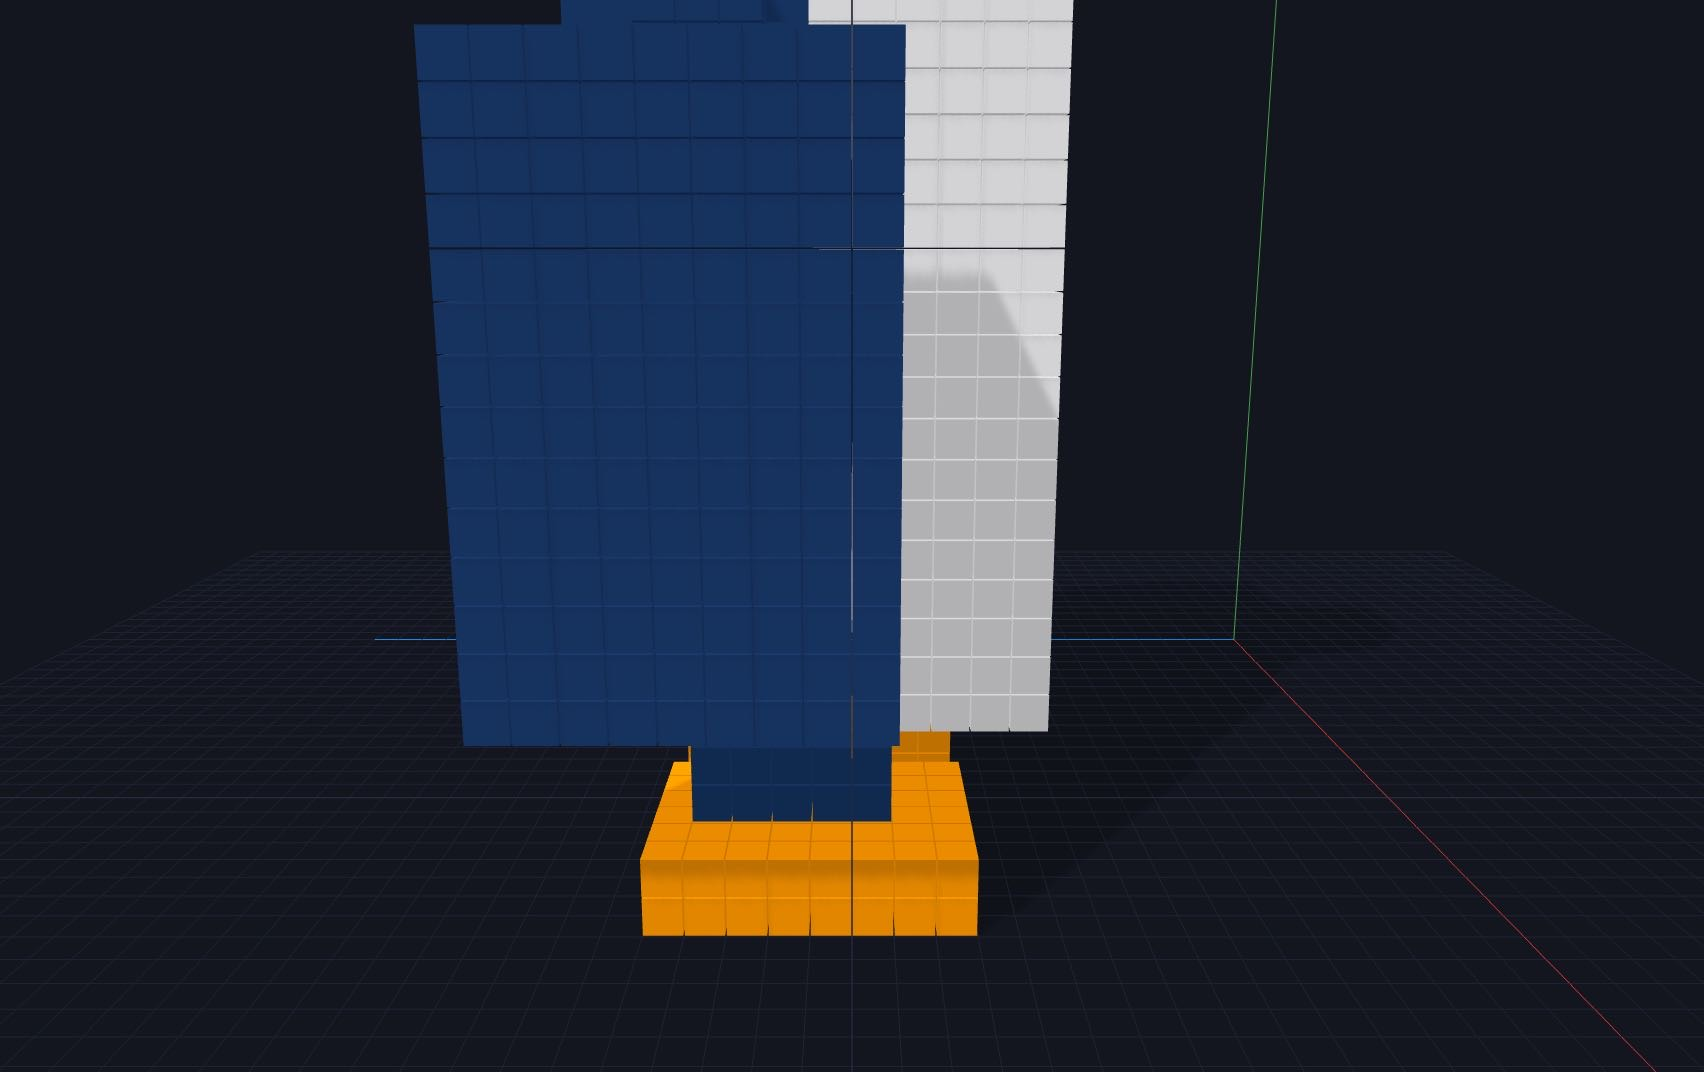
\includegraphics[width=\textwidth]{proposal-assets/penguin-render-left.jpg}
\end{minipage}%
\hfill
\begin{minipage}[t]{0.52\textwidth}
\lstinputlisting[basicstyle=\ttfamily\fontsize{5}{6}\selectfont]{proposal-assets/penguin-full-left.txt}
\end{minipage}

\vspace{8pt}

% TOP
\noindent\textbf{TOP View}\\[-4pt]
\rule{\textwidth}{0.4pt}

\noindent
\begin{minipage}[t]{0.45\textwidth}
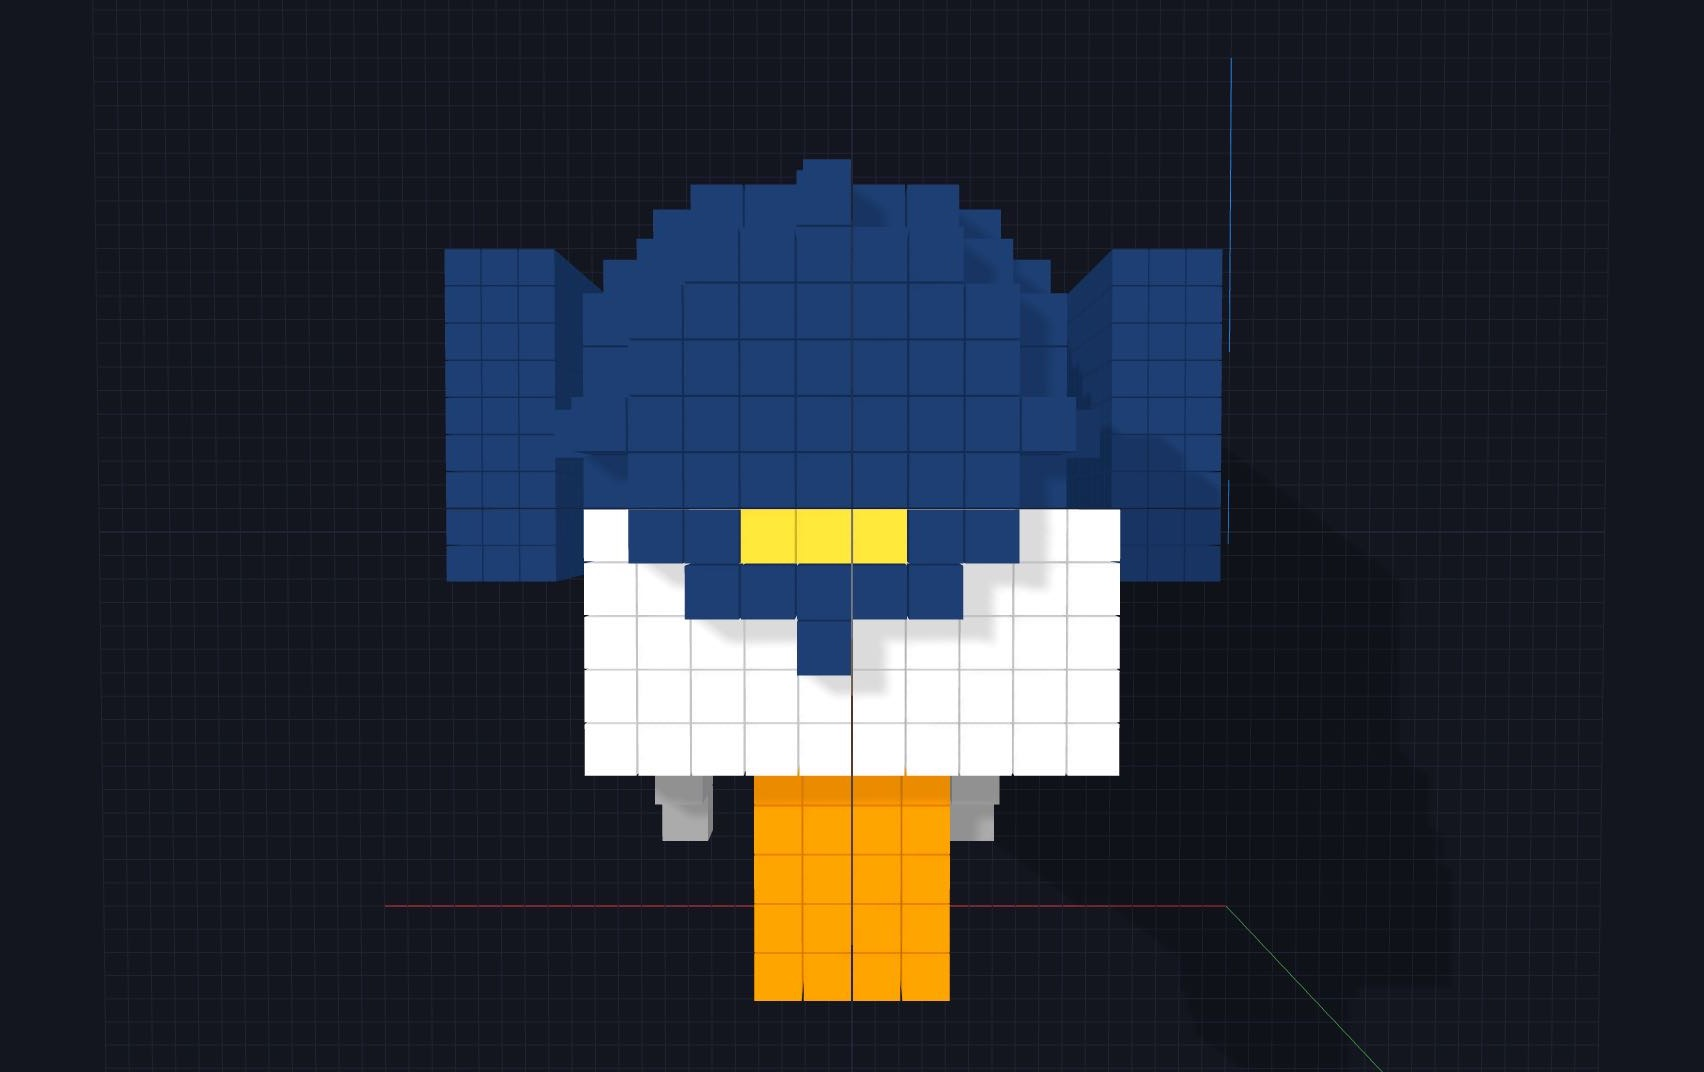
\includegraphics[width=\textwidth]{proposal-assets/penguin-render-top.jpg}
\end{minipage}%
\hfill
\begin{minipage}[t]{0.52\textwidth}
\lstinputlisting[basicstyle=\ttfamily\fontsize{5}{6}\selectfont]{proposal-assets/penguin-full-top.txt}
\end{minipage}

\end{document}
